\documentclass[a4paper, 12pt]{article}
\usepackage{graphicx, subcaption, amsmath, xcolor, pdfpages, geometry, fontspec, titlesec, titling}
\geometry{margin=1.0in}
\usepackage[os=win]{menukeys}
\AtBeginDocument{\AtBeginShipoutNext{\AtBeginShipoutDiscard}}

\newfontfamily\headingfont{Gill-Sans-MT-Condensed}[
    Path = ./fonts/,
    Extension = .TTF,
    UprightFont=*,
    Scale = 3
]
\let\Huge\headingfont

\begin{document}
\begin{titlepage}
	\begin{minipage}[t]{1\columnwidth}
		\begin{flushright}
       	\vspace{-0.6in}
       	
\includegraphics[width=0.3\textwidth]{MonextraNew.png}
			\vspace{0.5in}
		\par\end{flushright}
	\end{minipage}

	\begin{center}
		{\Huge Processing BTS Booklists Through the POS System}
	\end{center}
	\vspace{2em}
	\noindent
	\textbf{Created:} January 6, 2024
	\hfill
	\textbf{Updated:} \today
	\\\\\indent
	
	\tableofcontents
\end{titlepage}

\newpage
\section{Receiving ISI Shipments}
When an ISI order is delivered, the following steps must be taken to process the order.
\\
\\
On the Lotteries Terminal:
\begin{enumerate}
    \item Navigate to \menu{Instant Scratch It's > Receive Shipment}.
    \begin{figure}[h]
    \centering
        \hfill
        \begin{subfigure}{0.3\linewidth}
            \centering
            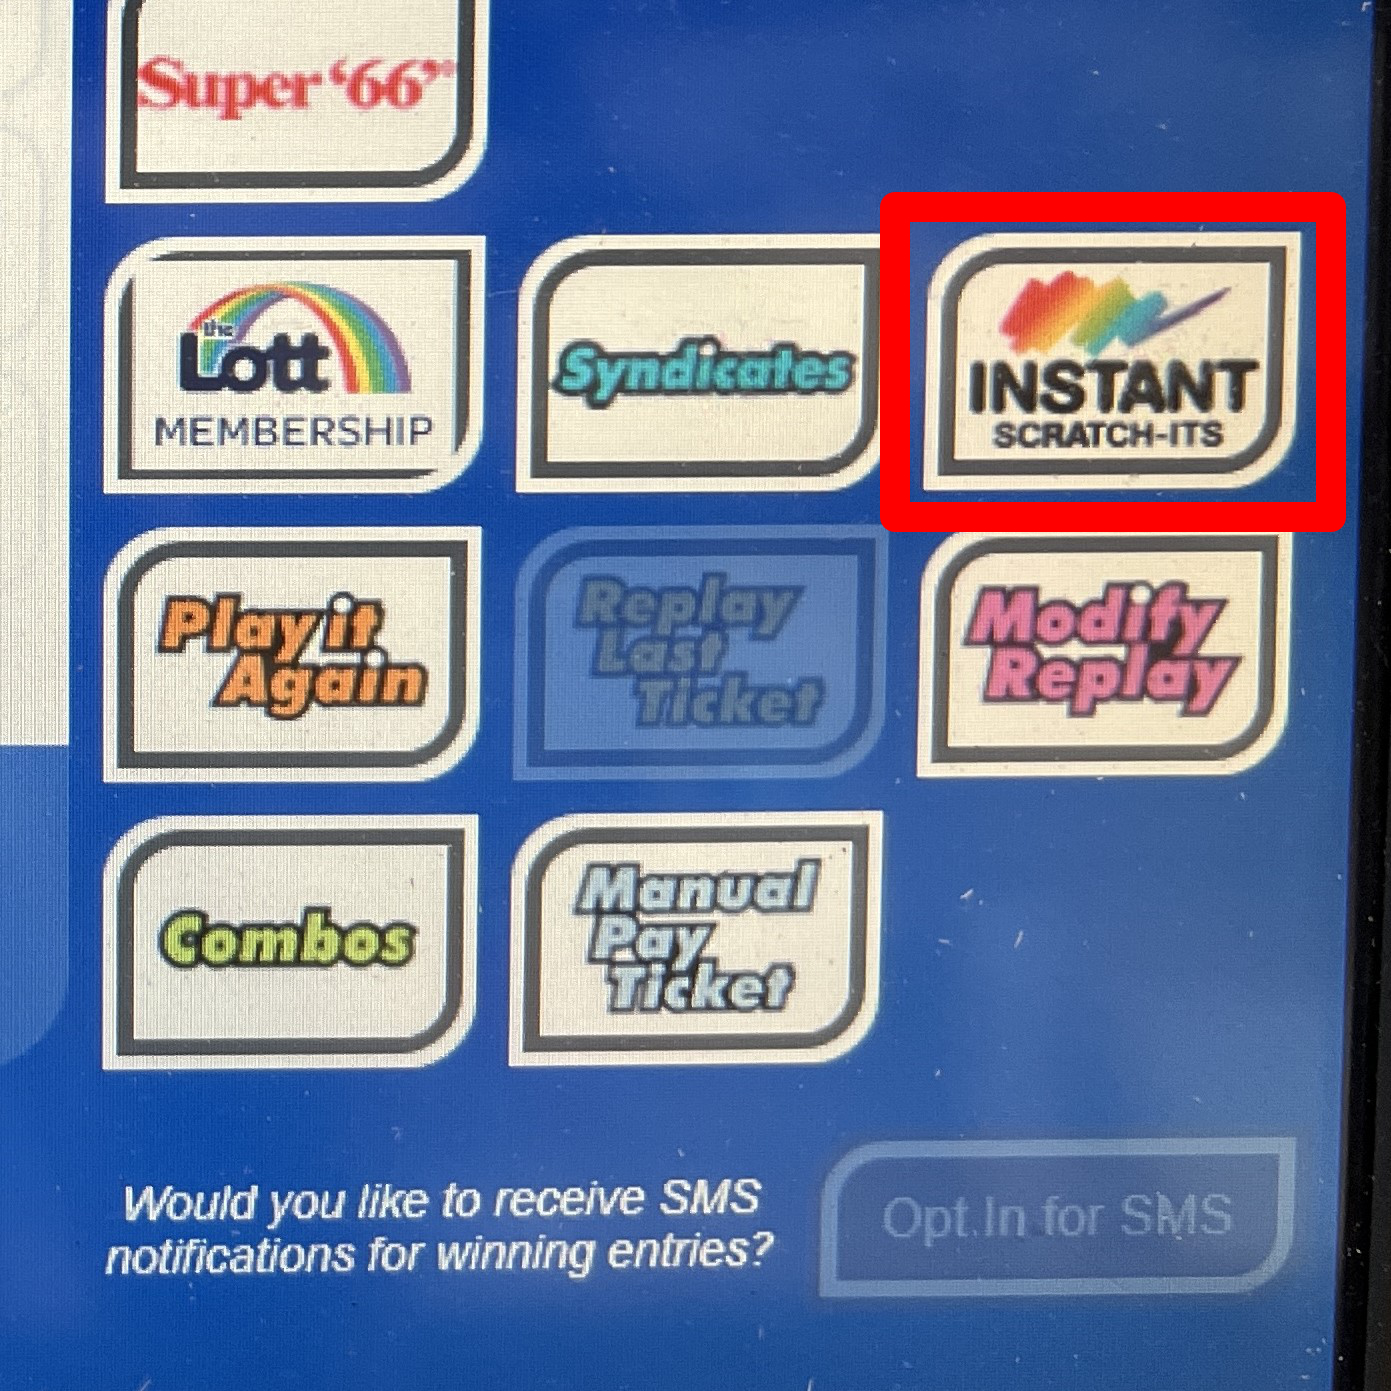
\includegraphics[width=\linewidth]{images/lotteriesmain.JPG}
        \end{subfigure}
        \hfill
        \begin{subfigure}[b]{0.3\linewidth}
            \centering
            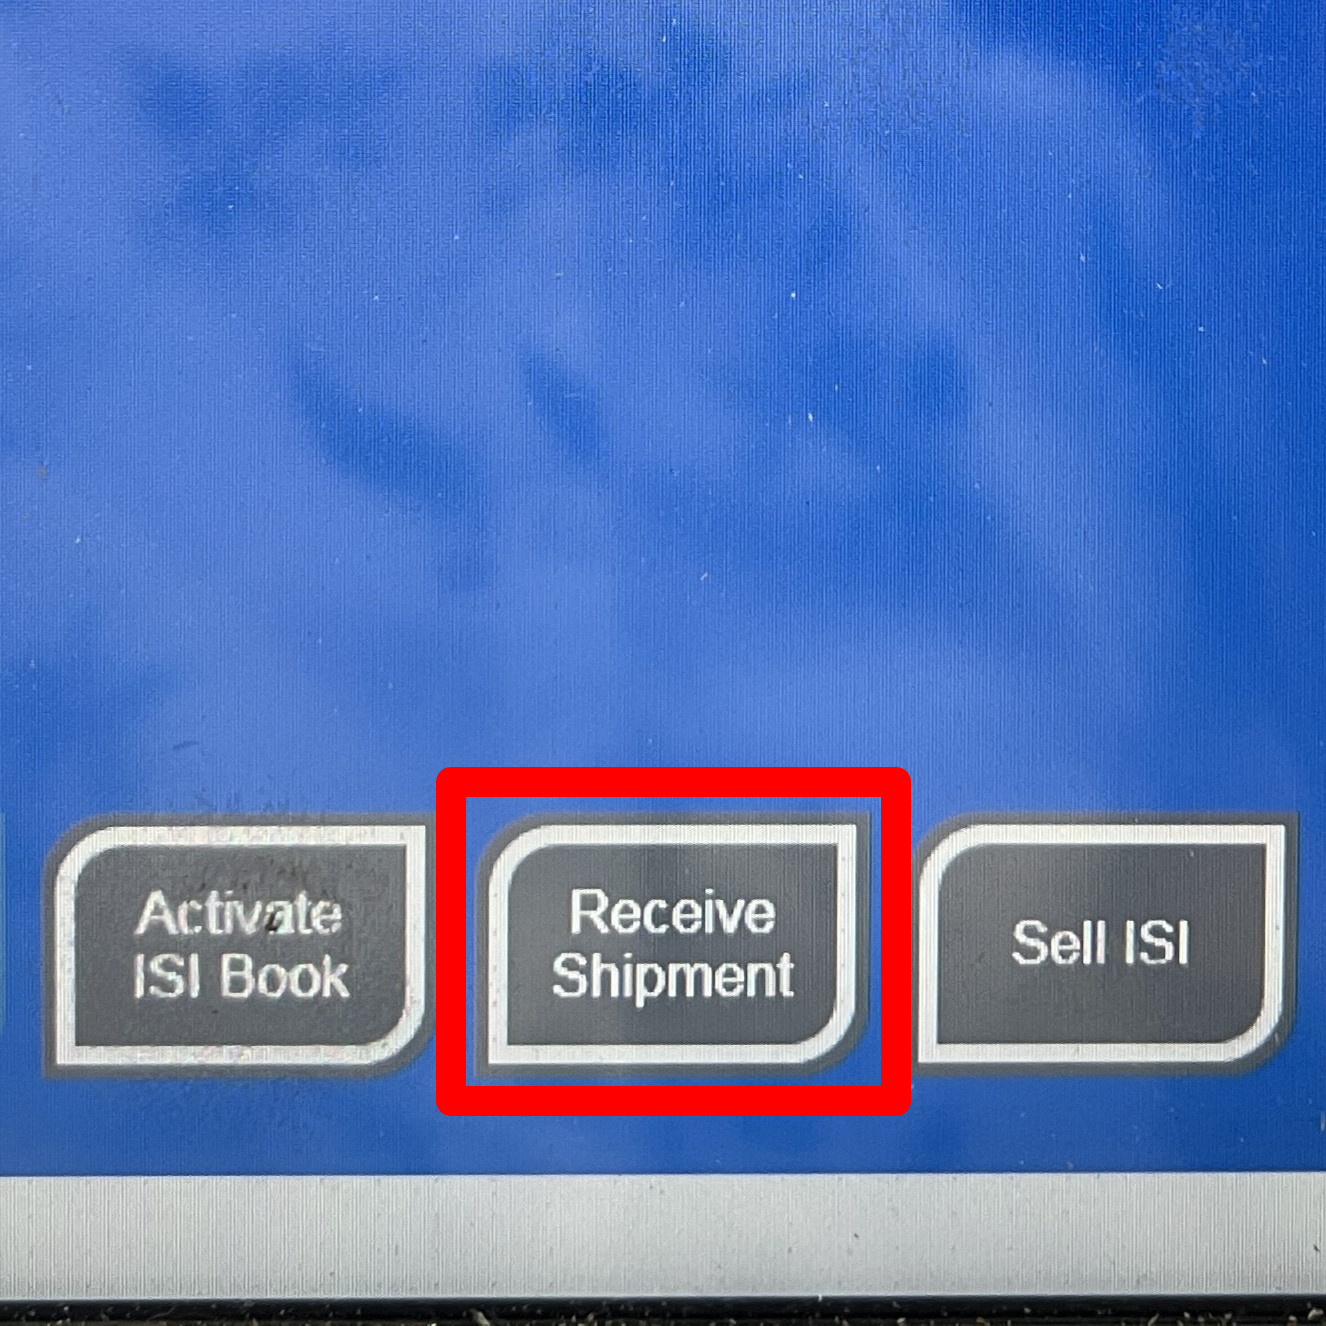
\includegraphics[width=\linewidth]{images/instantscratchits.JPG} 
        \end{subfigure}
        \hfill
        \begin{subfigure}[b]{0.3\linewidth}
            \centering
            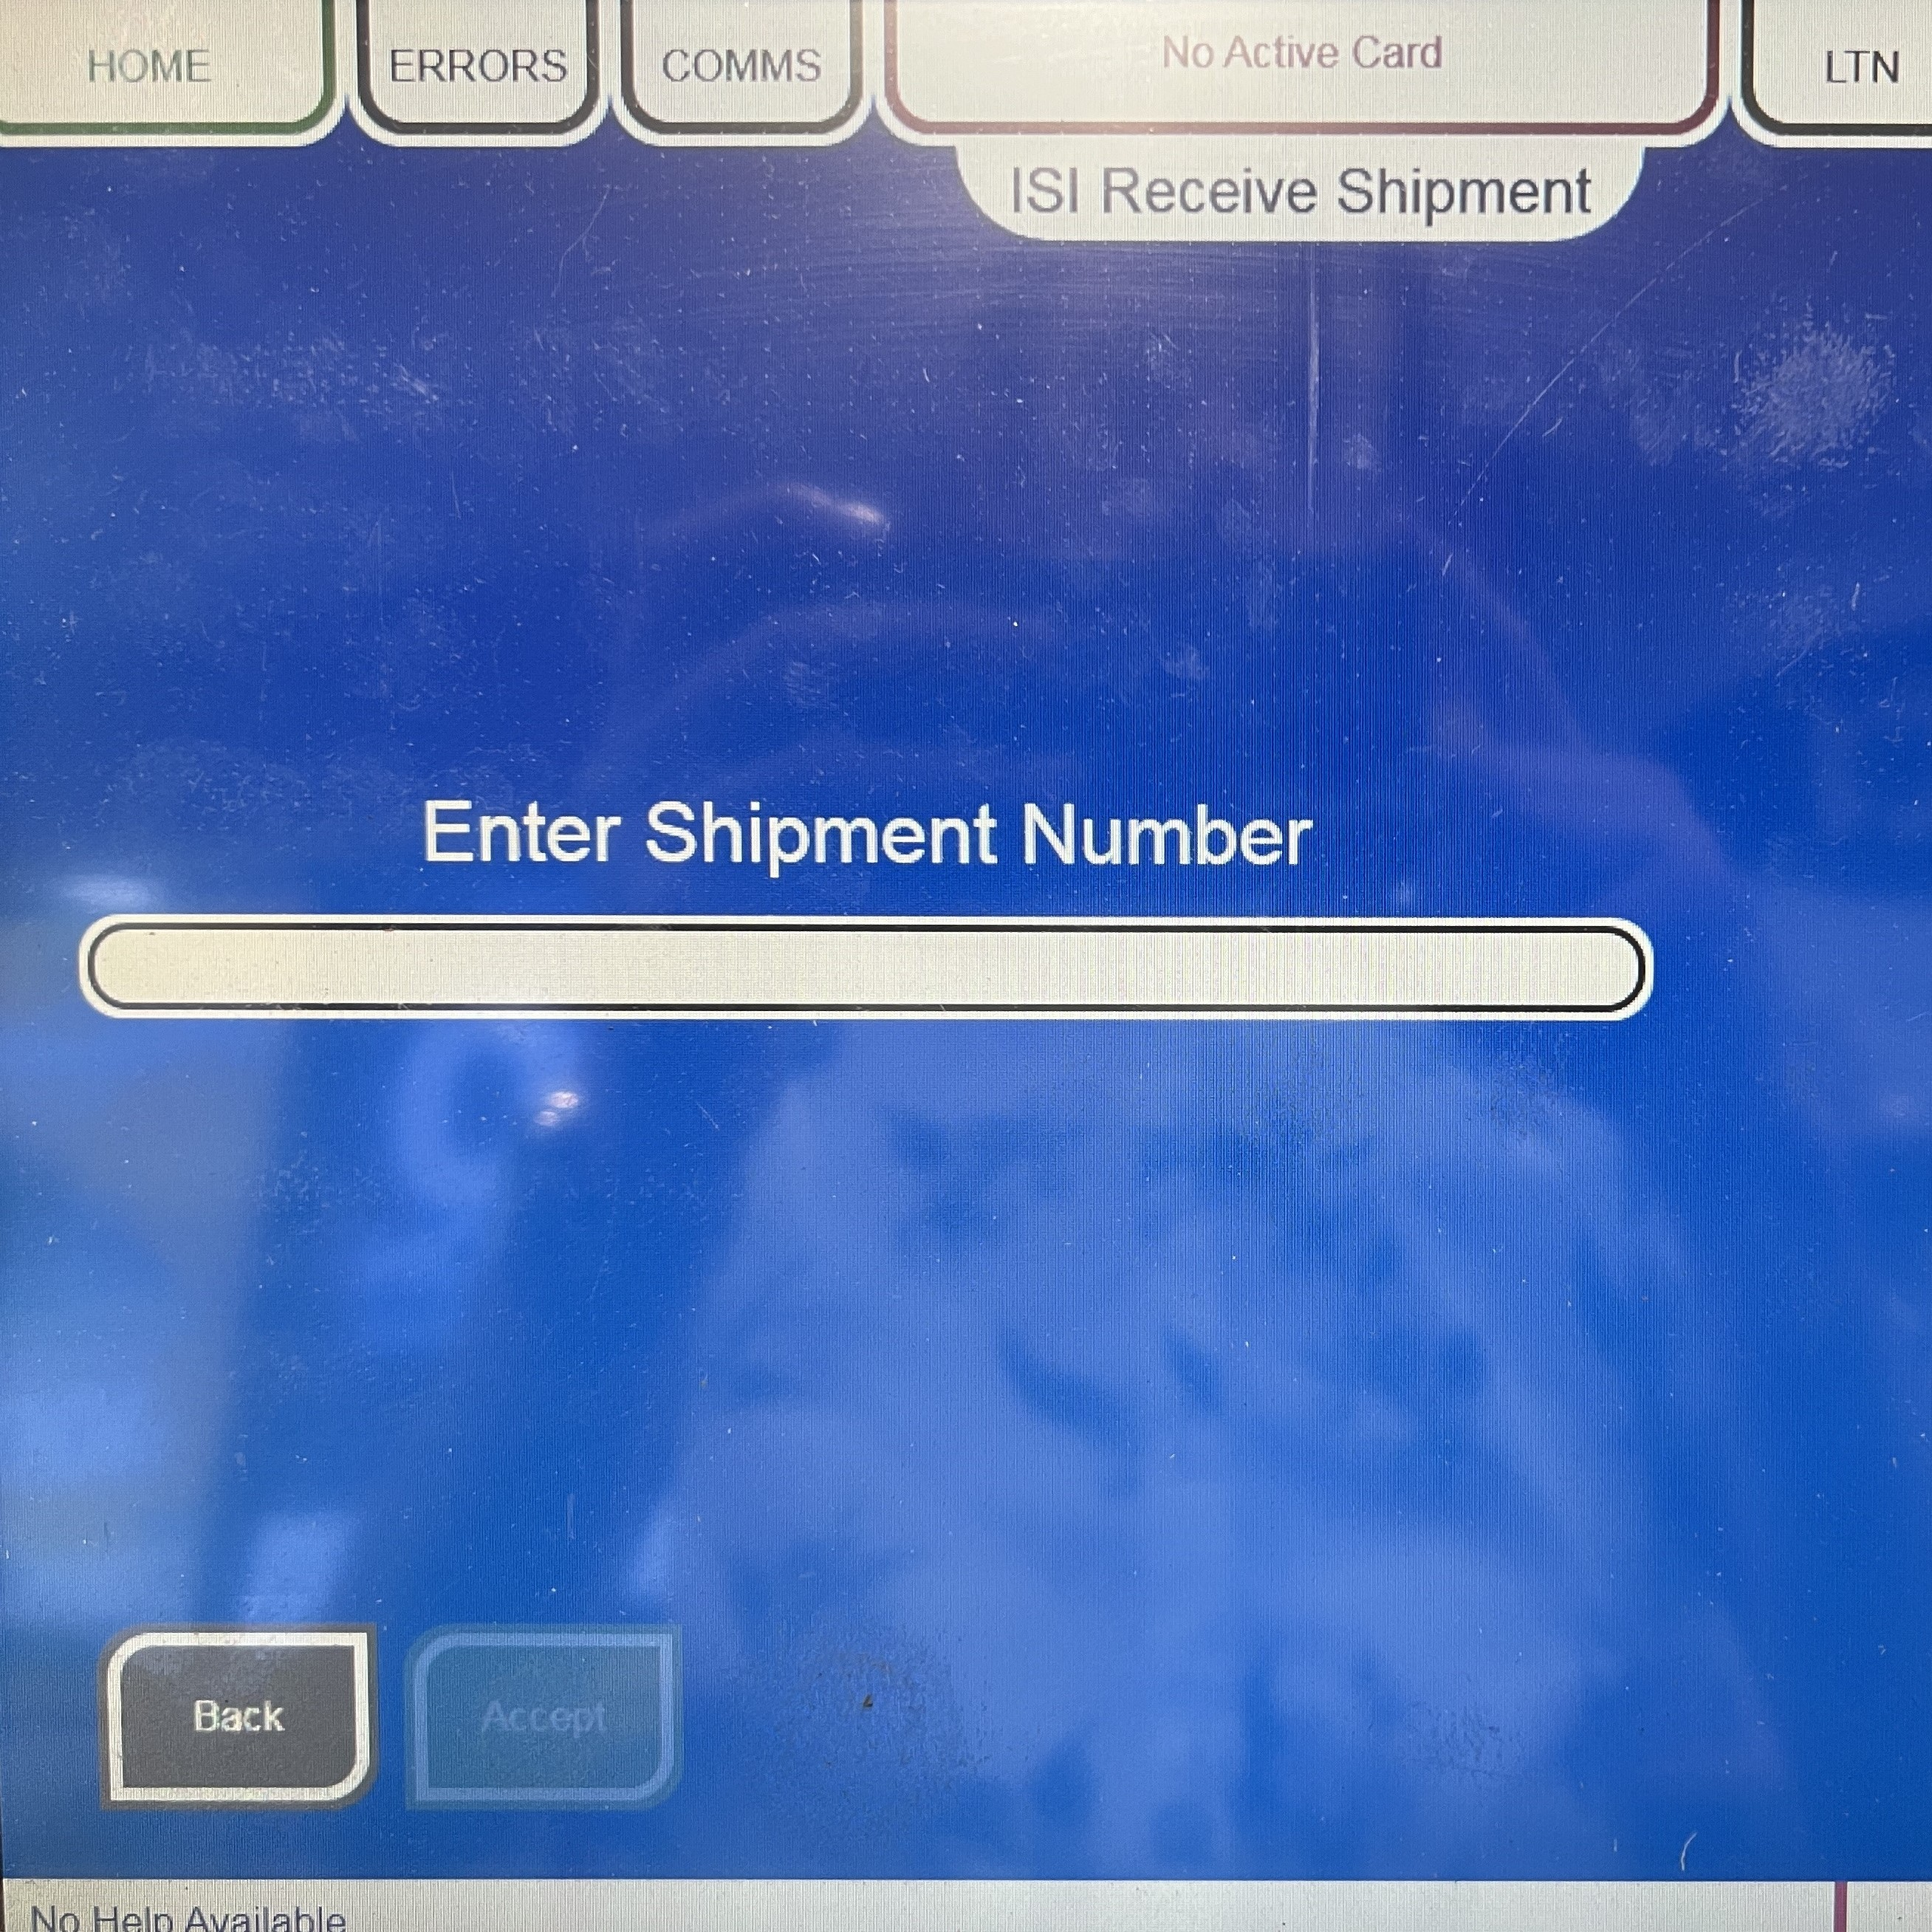
\includegraphics[width=\linewidth]{images/shipment.JPG} 
        \end{subfigure}
        \hfill
    \end{figure}
    \item On the \textit{Enter Shipment Number} screen, scan the shipment barcode located on the bottom of the packing slip that came with the ISI delivery.
    \begin{figure}[h]
        \centering
        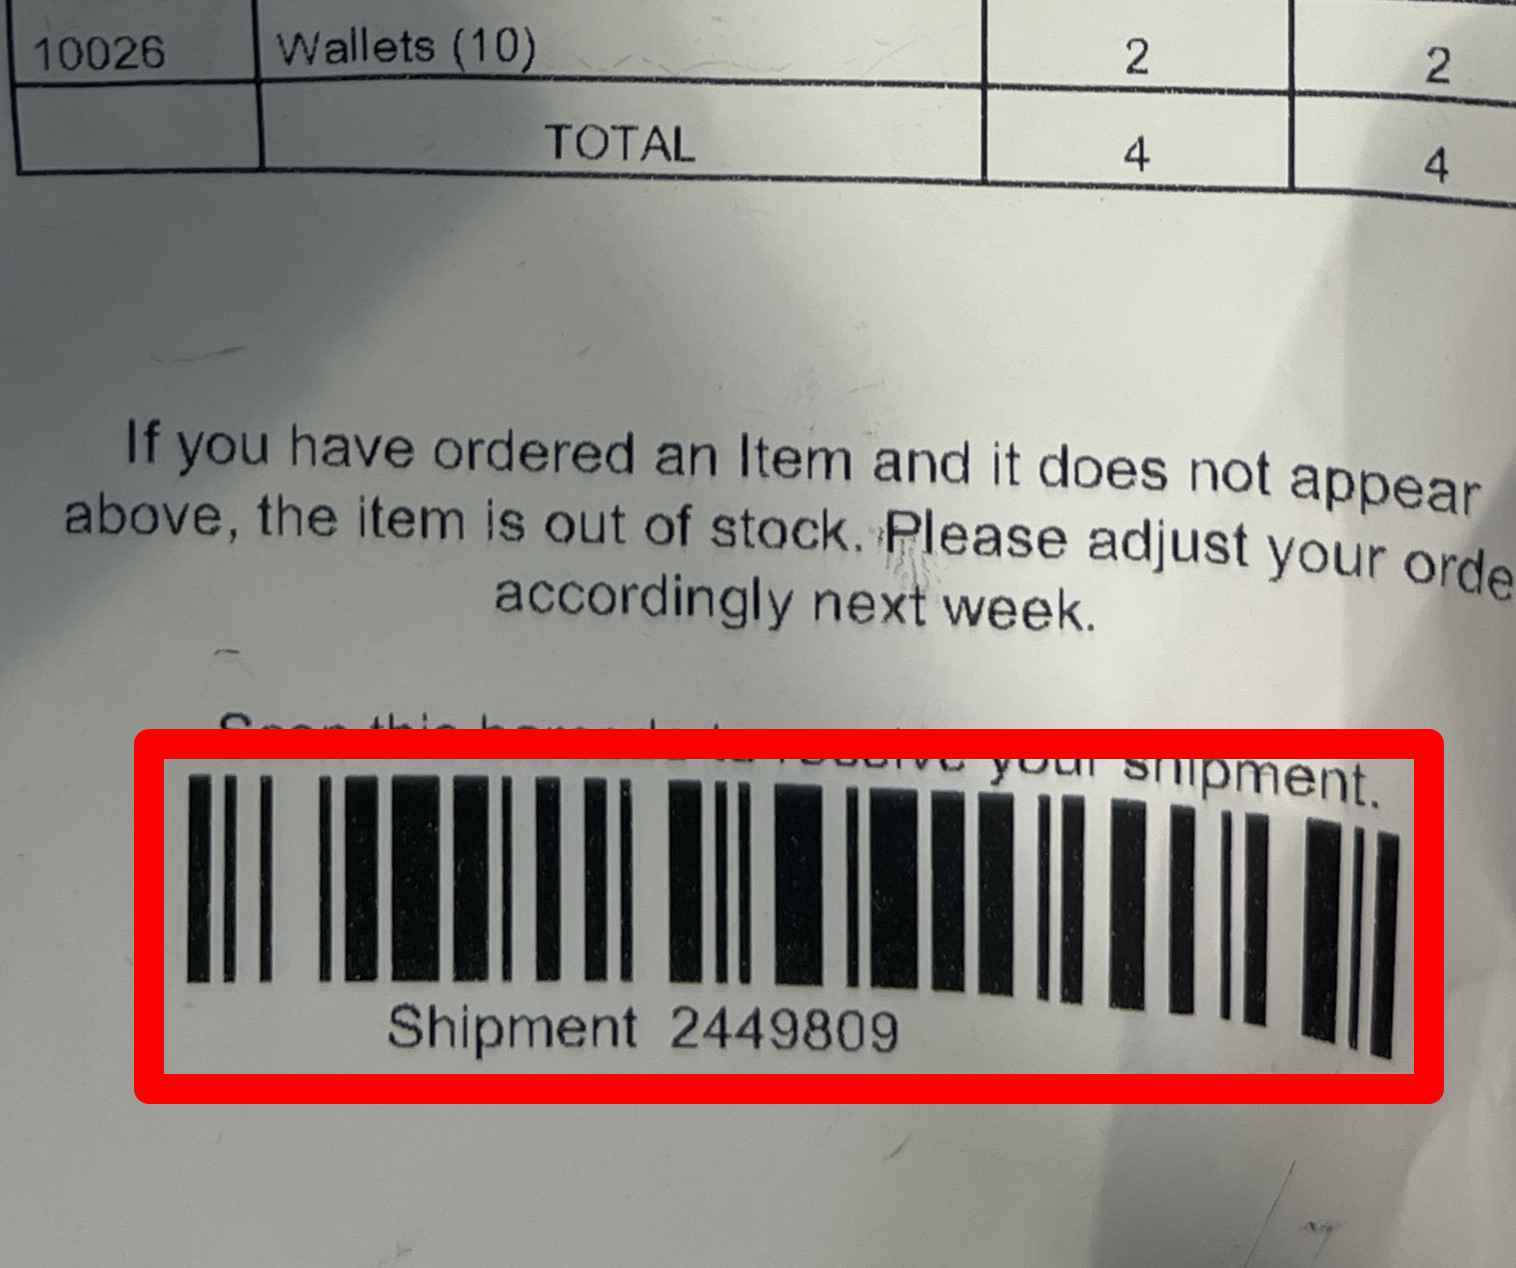
\includegraphics[width=0.5\linewidth]{images/isipackingslip.JPG}
    \end{figure}
\end{enumerate}

After the shipment has been received through the Lotteries Terminal, the packing slip must be scanned and emailed.
\begin{enumerate}
    \item Place the packing slip/s face down on the copier glass.
    \\
    \begin{flushright}
        \textbf{\textit{continued...}}
    \end{flushright}
    \newpage
    \item Press \menu{Email}.
    \begin{figure}[h]
        \centering
        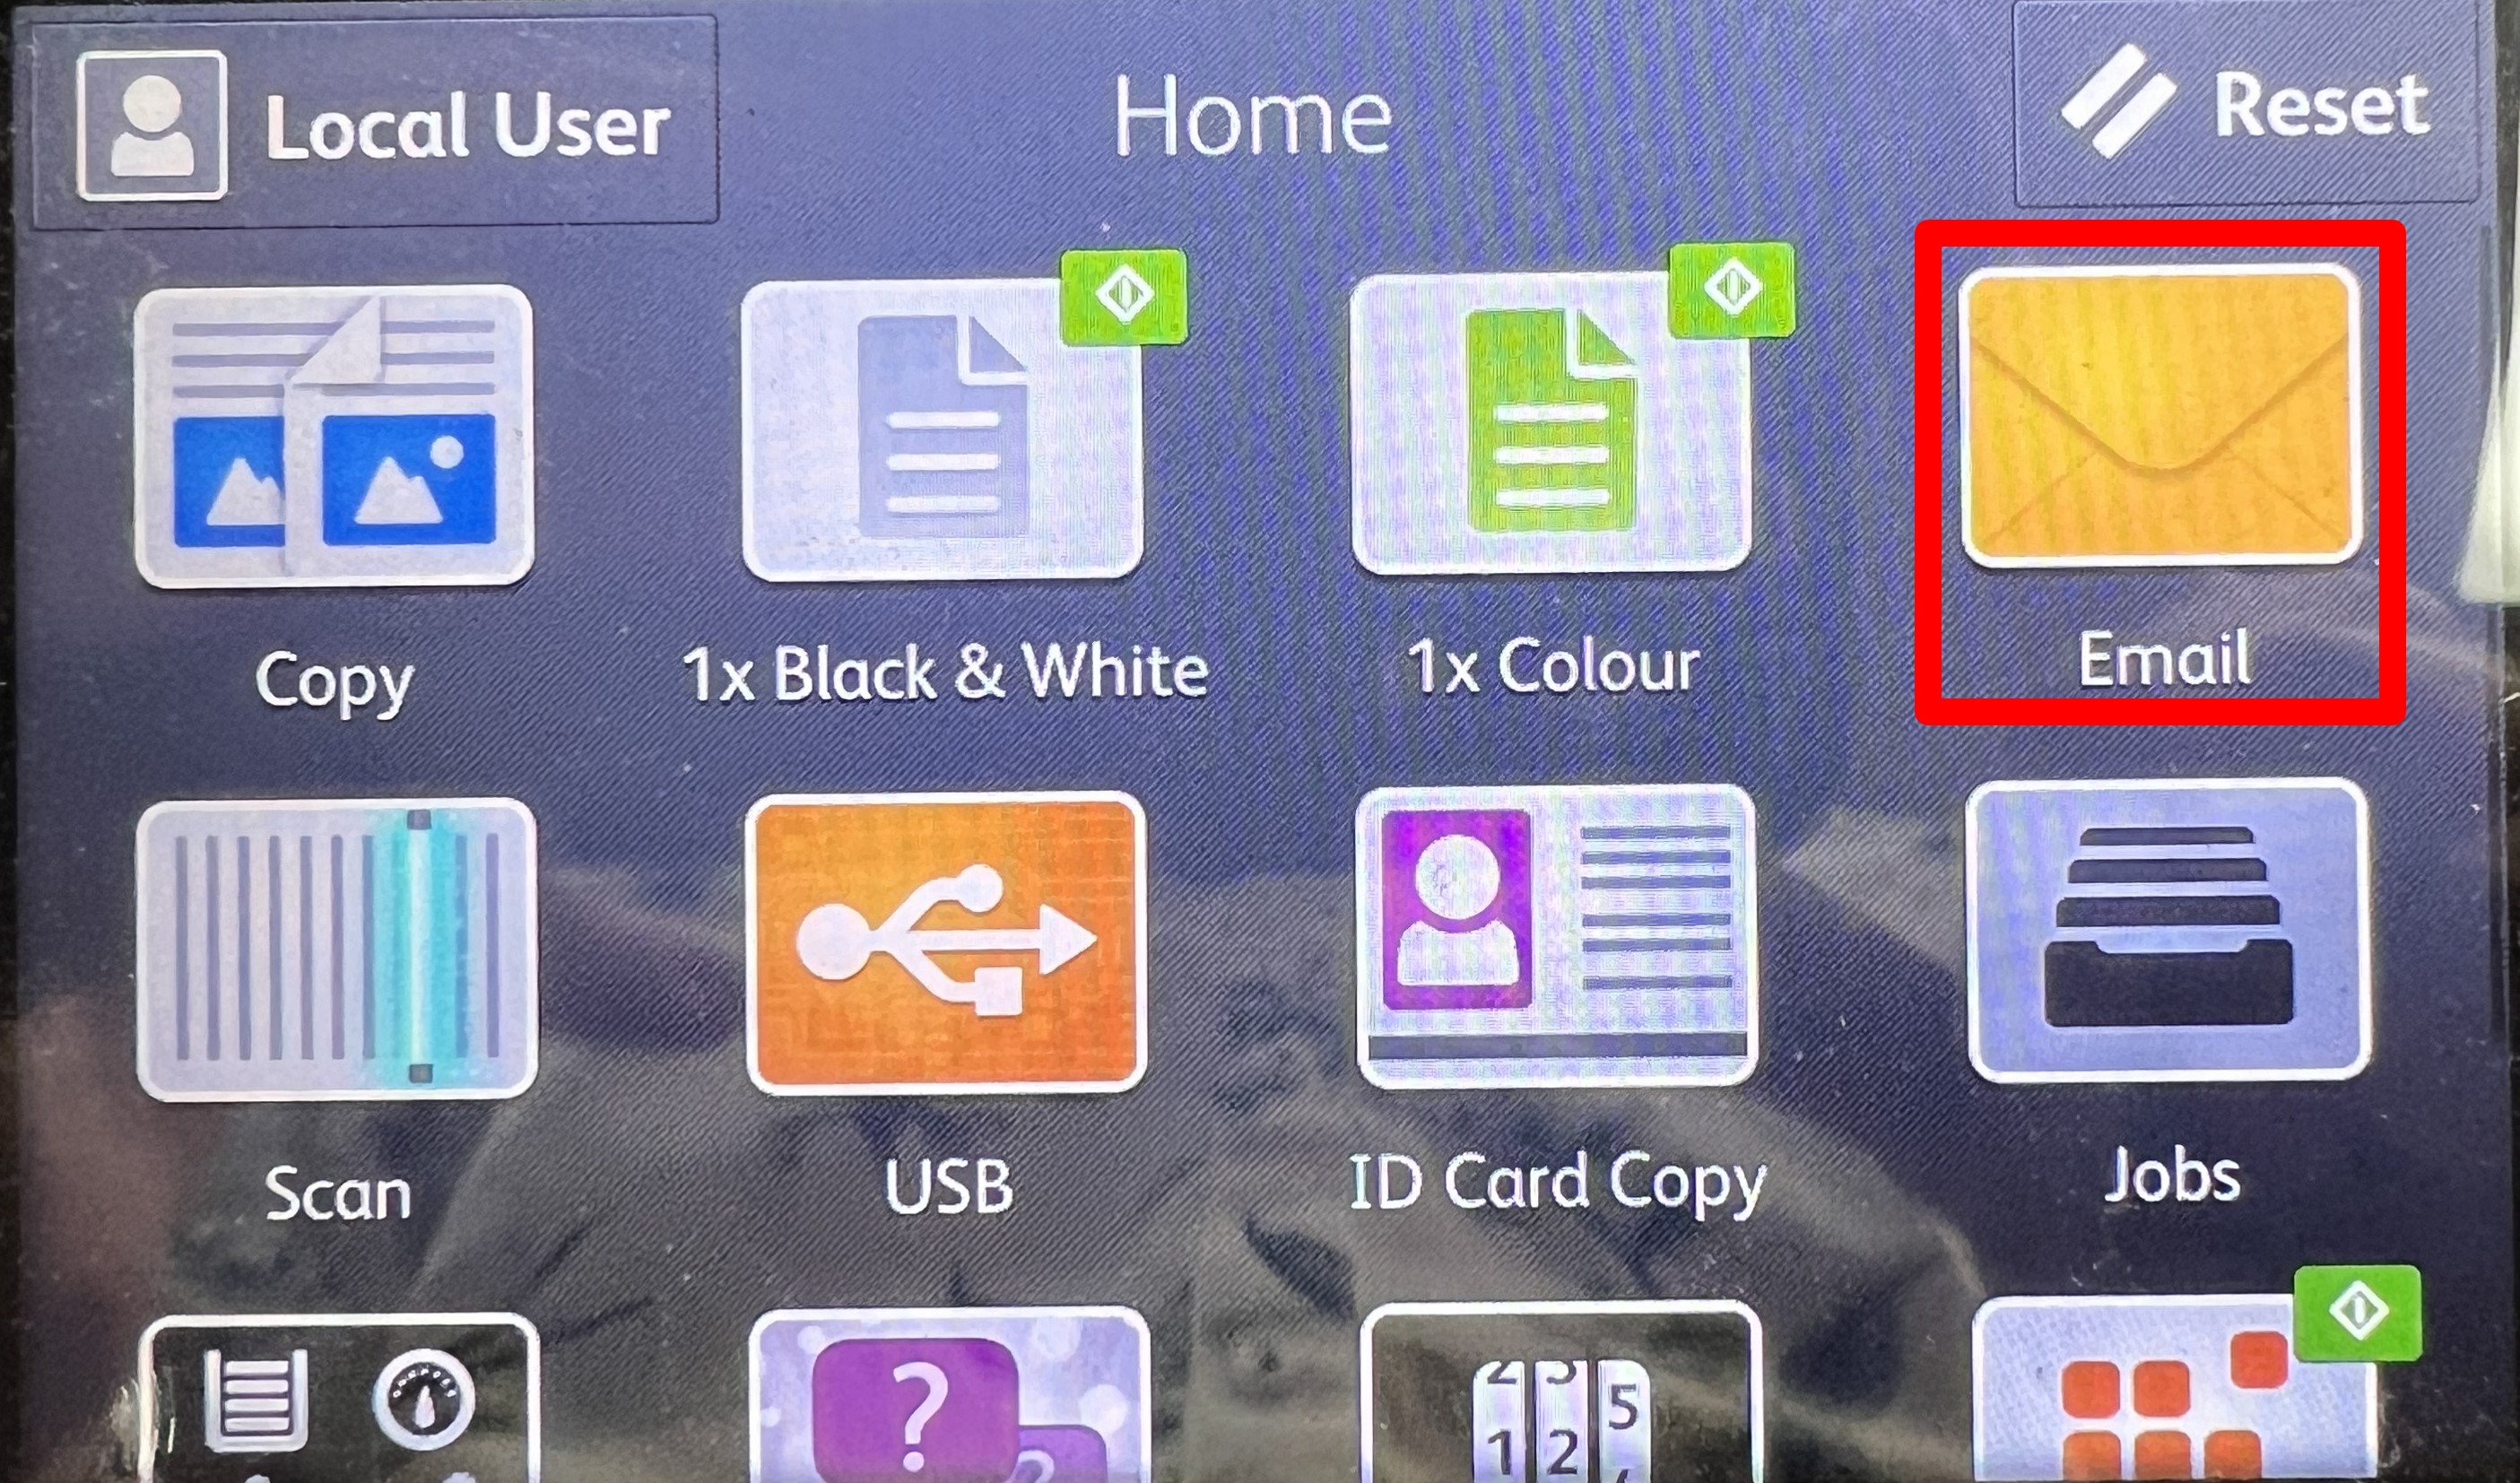
\includegraphics[width=0.5\linewidth]{images/printermain.JPG}
    \end{figure}
    \item Select the \textit{To} box and start typing Connor, select the email address  \\ \texttt{connor@nextramorayfield.com} when it pops up.
    \begin{figure}[h]
        \centering
        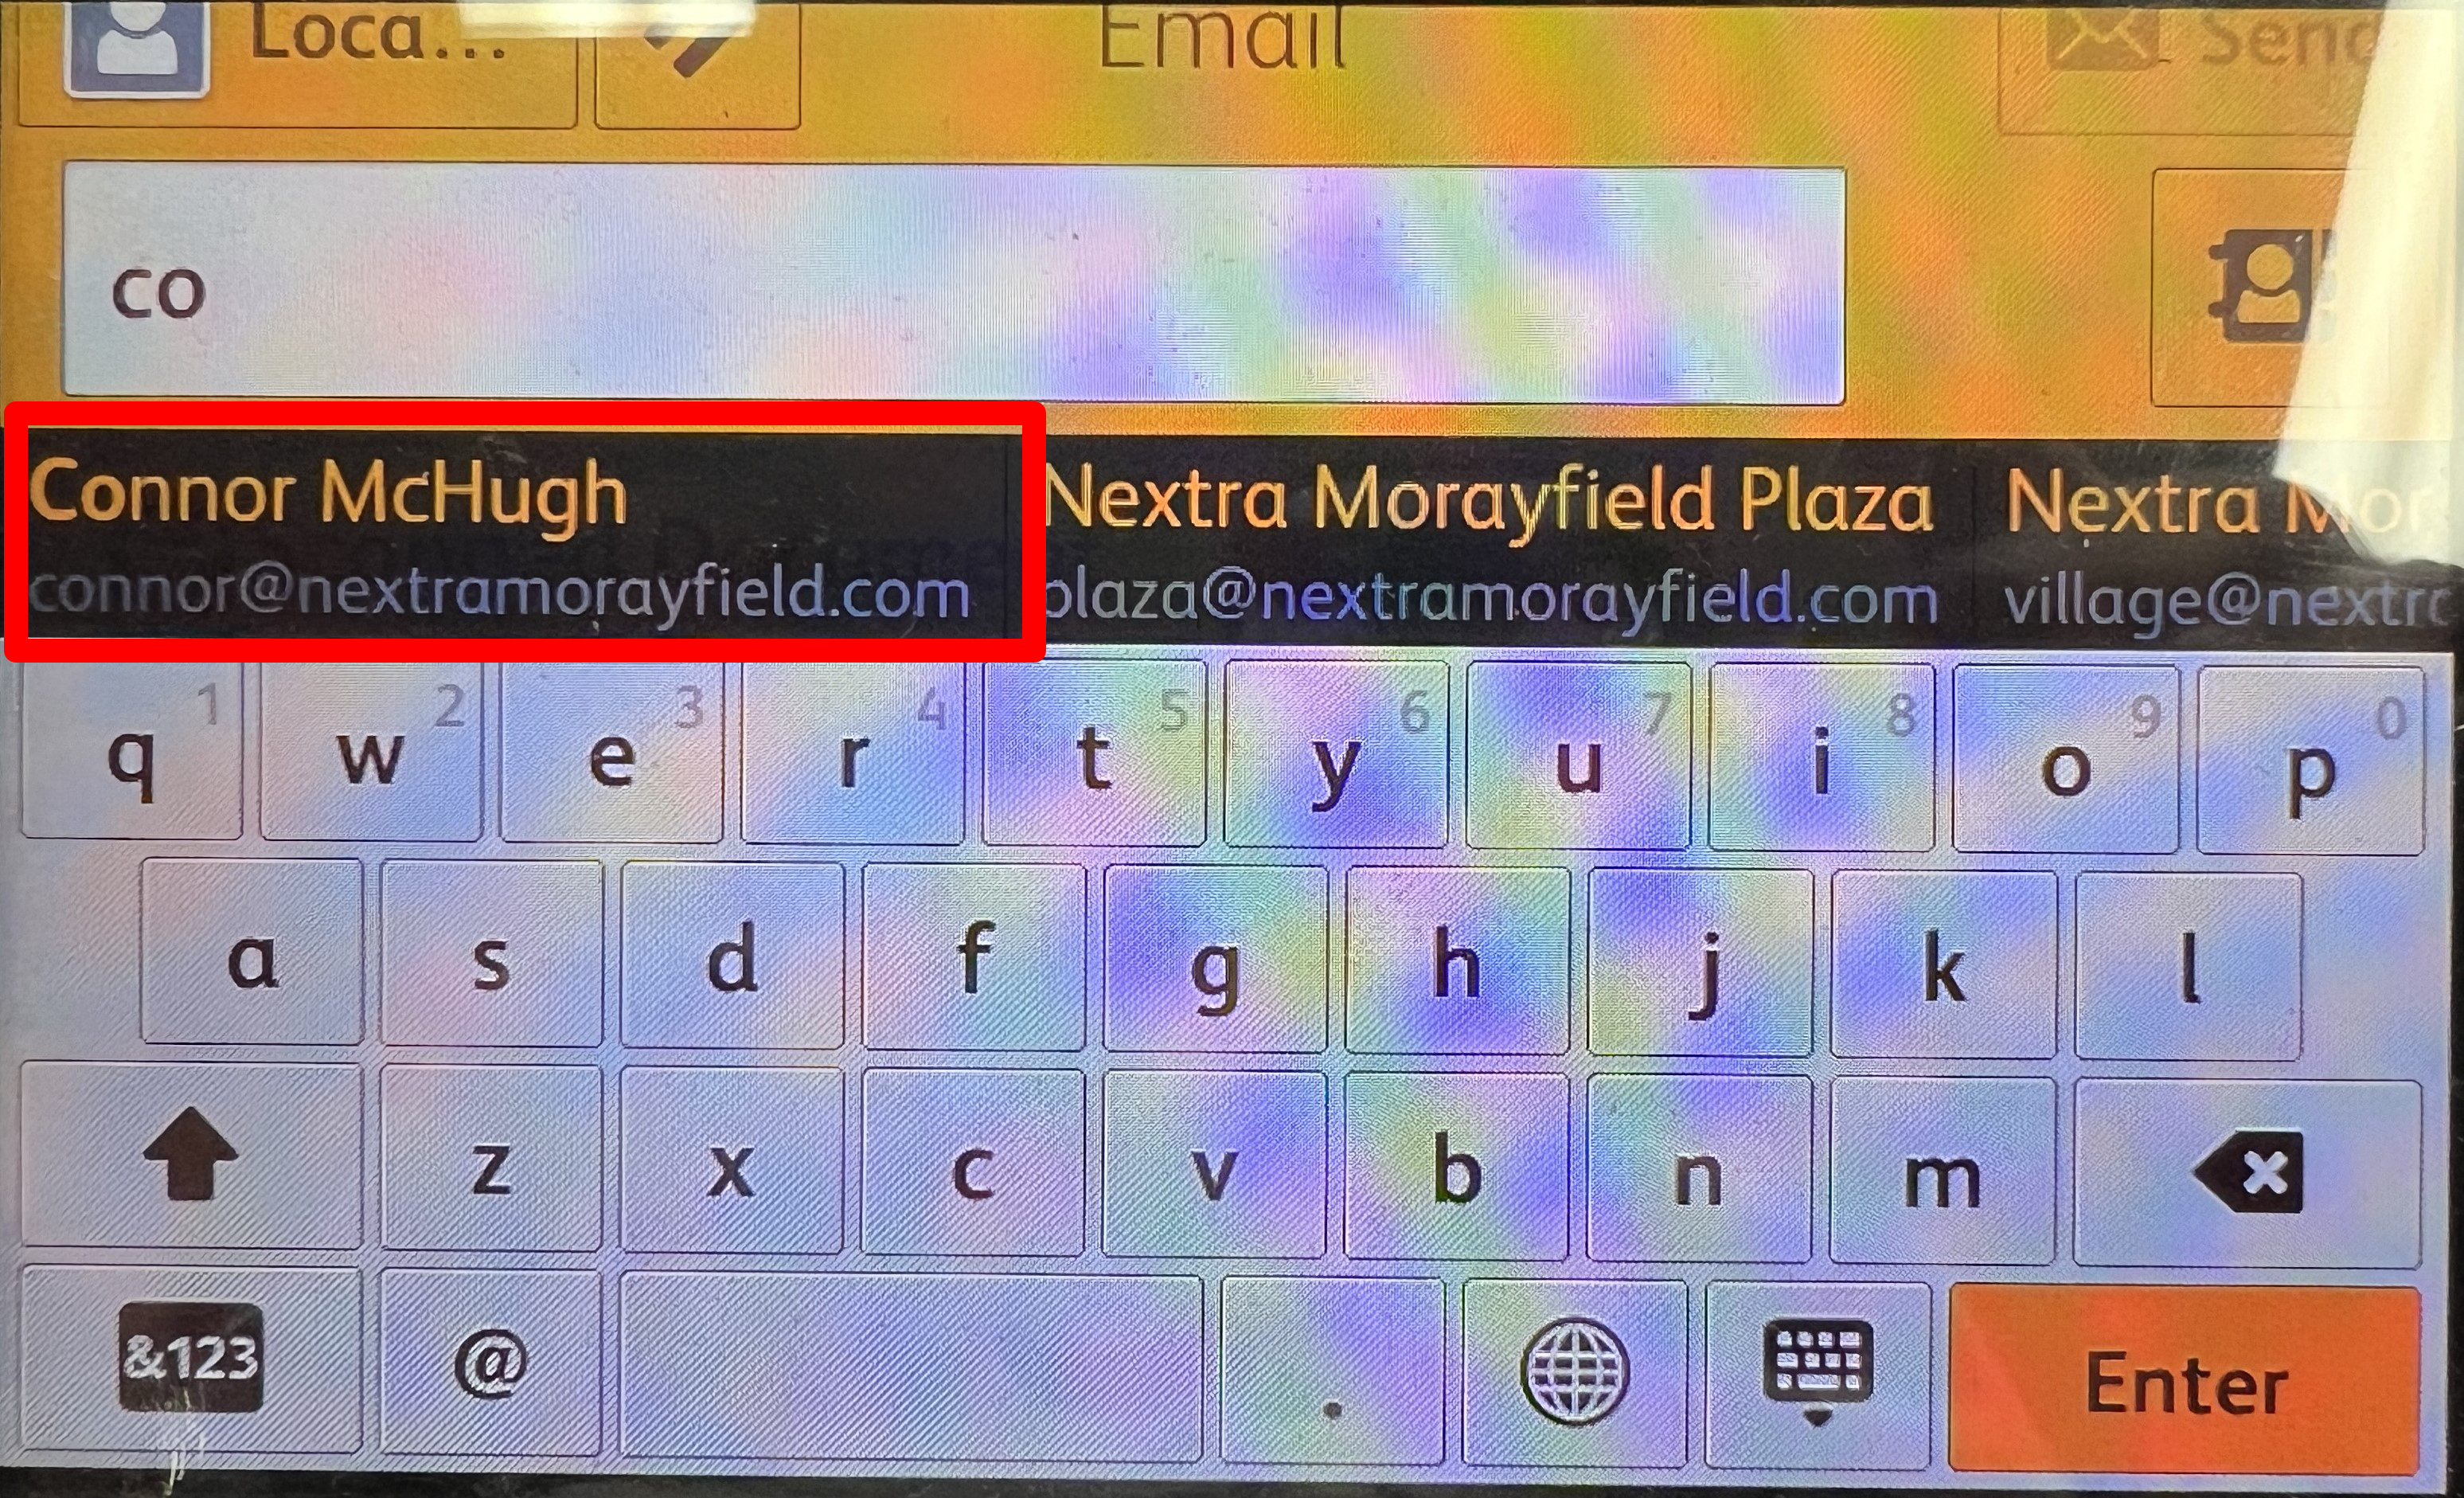
\includegraphics[width=0.5\linewidth]{images/email.JPG}
    \end{figure}
    \item Press \menu{Send}.
    \begin{figure}[h]
        \centering
        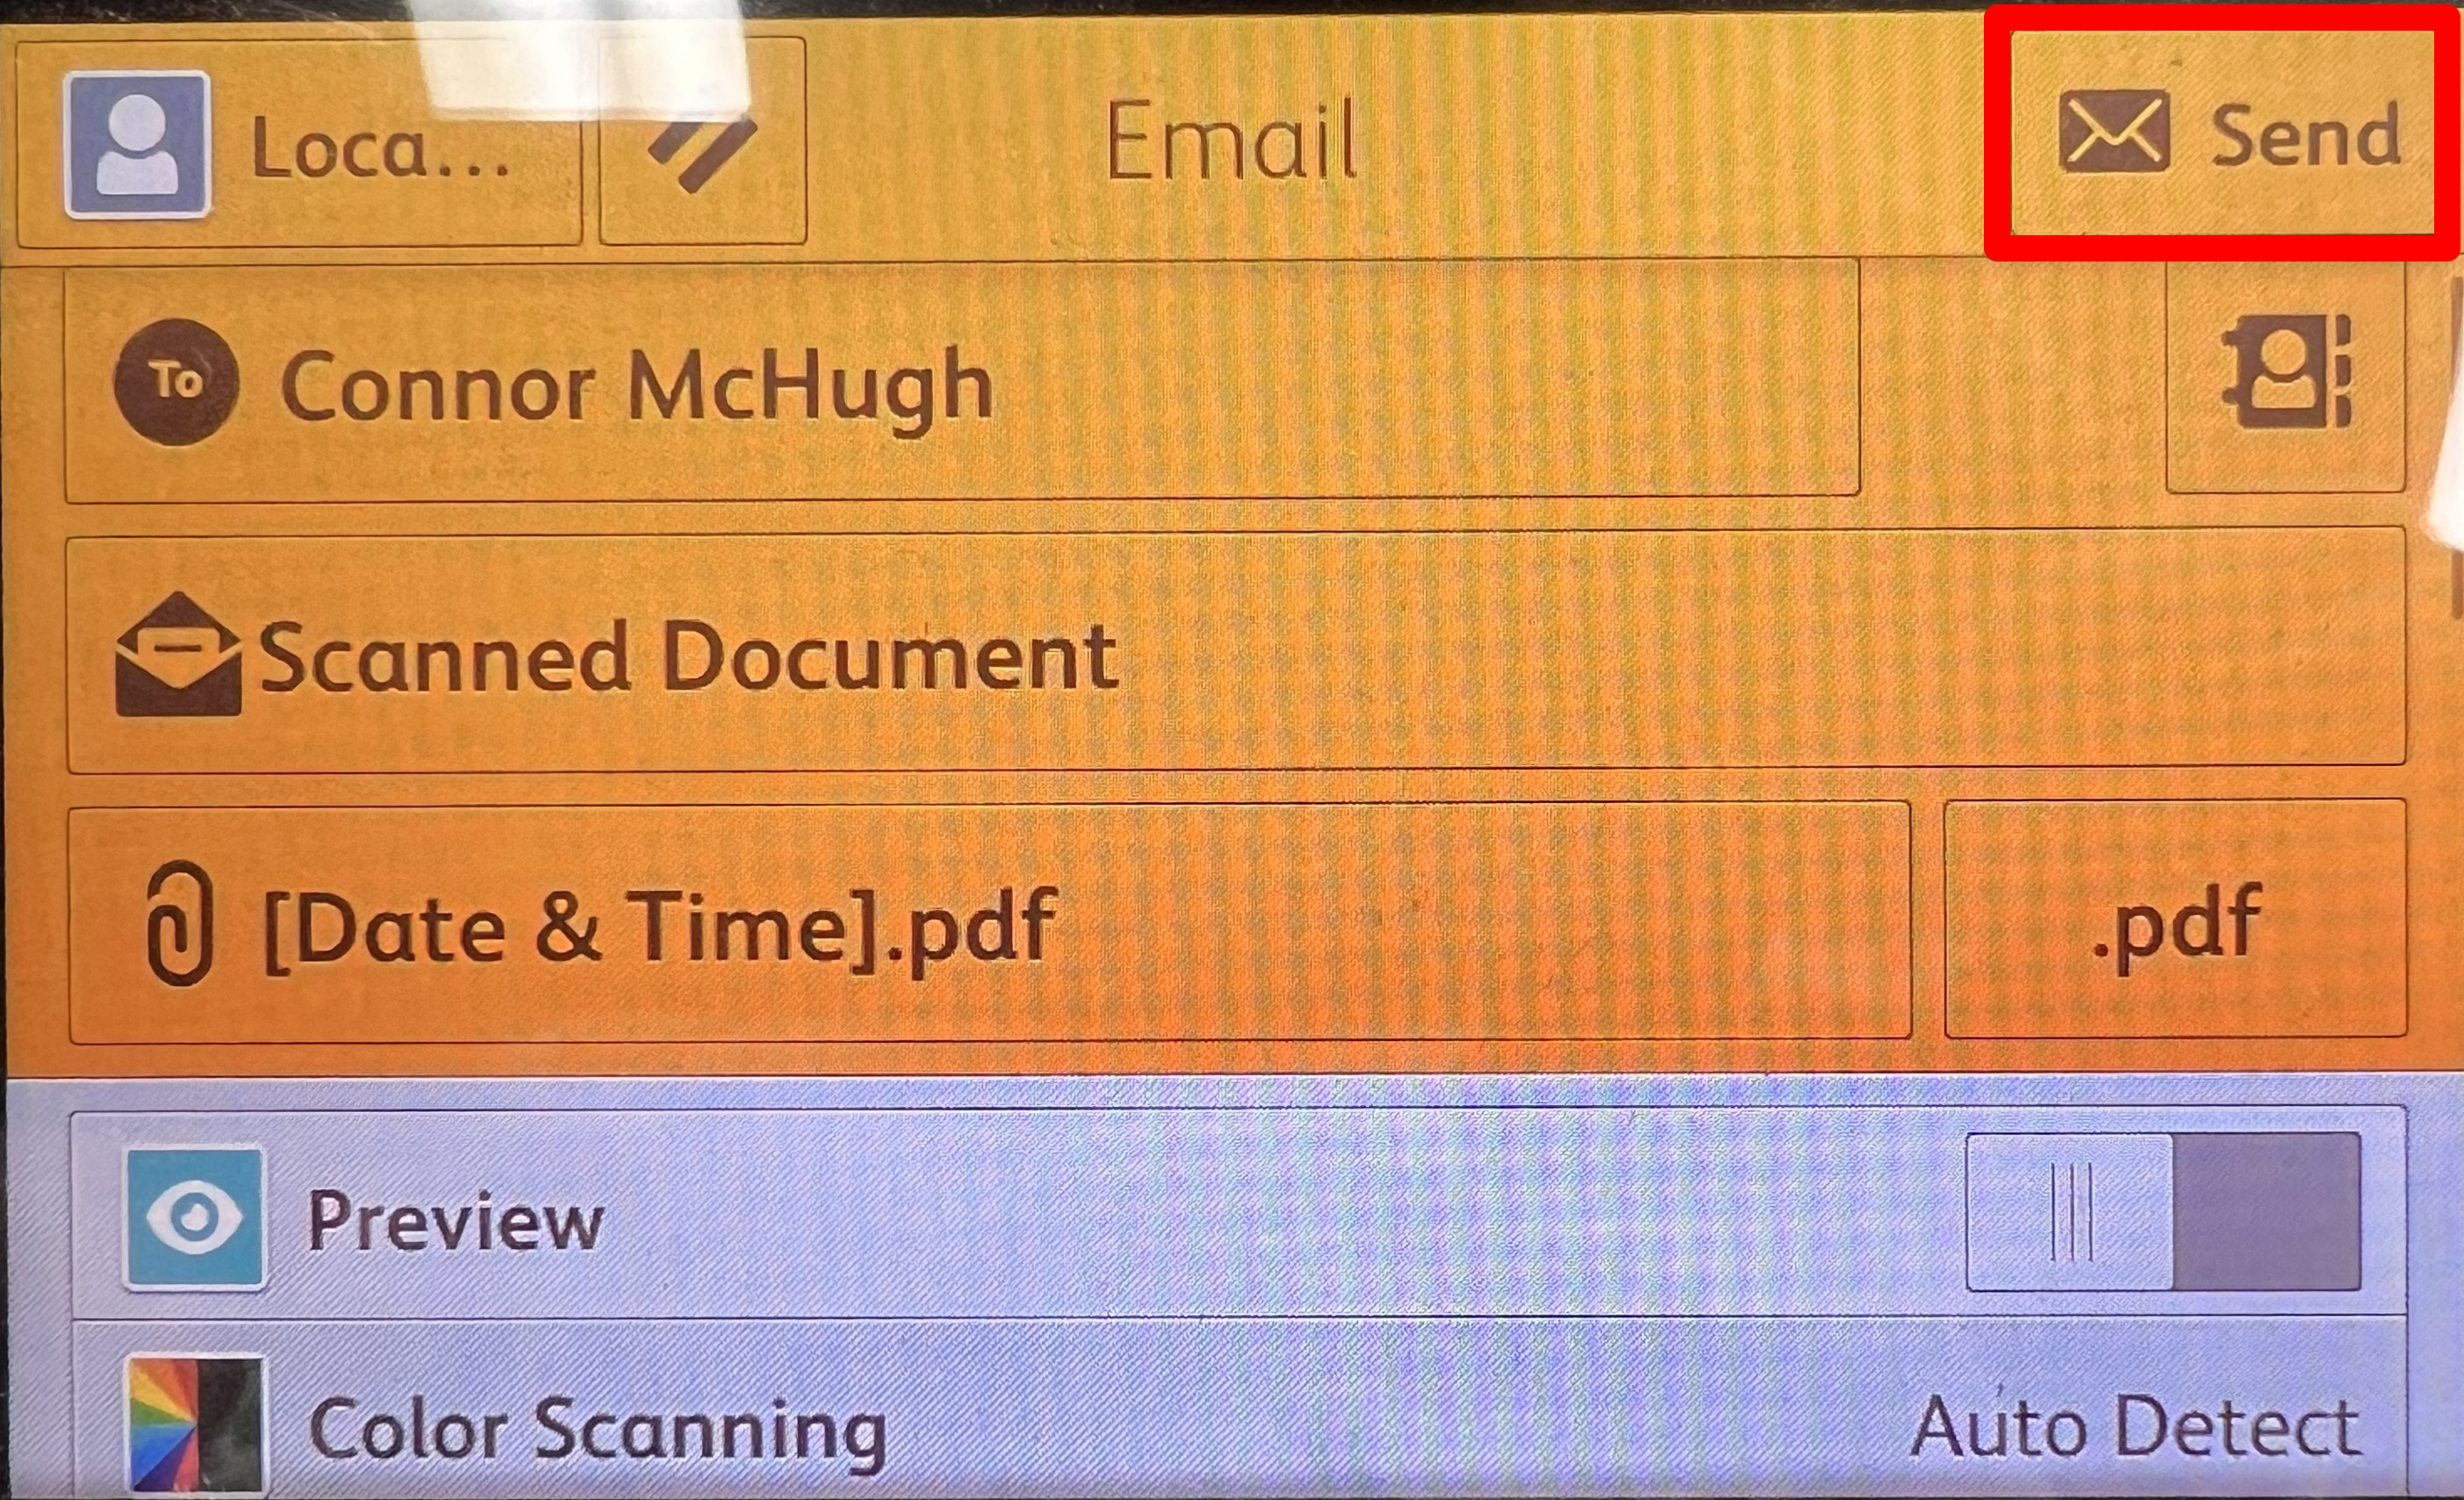
\includegraphics[width=0.5\linewidth]{images/send.JPG}
    \end{figure}
\end{enumerate}
Once the packing slip has been scanned and sent, it as well as the shipment summary printed by the terminal can be discarded.

\newpage
\section{Withdrawing ISI Books}
When you need to withdraw ISI books from the safe into the counter drawer, you must count the number of each value of book and write them into the ISI count book in the following format:
\\ \\
\hspace*{1cm}%
\begin{minipage}{.8\textwidth}%
   Day \& Date \\
   \textbf{C/O =} Previous day's count \\
   \textbf{New =} Qty $\times$ Value = \$ Total of books of value \\
   \textbf{Total Books = } Total number of books taken out \\
   \textbf{Total \$ =} Total \$ value of books taken out \\
   \textbf{New C/O =} C/O + Total \\
\end{minipage}%
\\
For example:
\\ \\
\hspace*{1cm}
\begin{minipage}{.8\textwidth}
   Monday 01/01/2024 \\
   \textbf{C/O =} 15,000 \\
   \textbf{New =} \\
   2 $\times$ \$1 = 400 \\
   4 $\times$ \$5 = 1,000 \\
   3 $\times$ \$10 = 900 \\
   \textbf{Total Books = 9} \\
   \textbf{Total \$ =} 2,300 \\
   \textbf{New C/O =} 17,300 \\
\end{minipage}
\\
Have another team member double count the quantities of each book value, the total books, and double check the adding and totals. 
\color{red} \textbf{This is extremely important as there is no way to confirm how many books have been taken out once they go into the drawer.} \color{black}


\newpage
\section{EOM ISI Reconciliation}
On the last day of each month, the unactivated ISI books must be reconciled. Each month, a reconciliation form will be provided, following are the steps to complete this form:

\begin{enumerate}
    \item Write the name of the team member completing the reconciliation
    \begin{figure}[h]
        \centering
        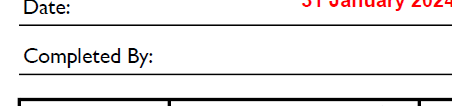
\includegraphics[width=0.5\linewidth]{images//reconsheet/completedby.png}
    \end{figure}
    \item Once you are sure that you will not need to withdraw any more ISI books, you can count the safe. Count the number of each game type, match up the game number on the book with the game number on the form, and write the number of books in the \textit{Safe} column.
    \begin{figure}[h]
    \centering
        \hfill
        \begin{subfigure}[b]{0.3\linewidth}
            \centering
            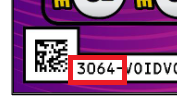
\includegraphics[width=\linewidth]{images/reconsheet/isiticket.png} 
        \end{subfigure}
        \hfill
        \begin{subfigure}[b]{0.45\linewidth}
            \centering
            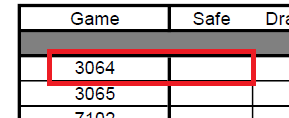
\includegraphics[width=\linewidth]{images/reconsheet/safebook.png} 
        \end{subfigure}
        \hfill
    \end{figure}
    \item Once you are sure that you will not need to top-up the ISI dispenser/s, you can count the drawer. Follow the same procedure as used to count the safe to complete the \textit{Drawer} column. \textbf{If there are any books in the drawer that have been activated, do not include these in your count.}
    \item For each game, add the \textit{Safe} and \textit{Drawer} columns to complete the \textit{Total} column.
    \item On the Lotteries Terminal, navigate to \menu{Admin > Reports > ISI Inventory}, ensure that the \menu{Summary} option is selected, and press \menu{Generate Report} then \menu{Print} the report.
    \item Use the figures in the \textit{RECEIVED} column of the printed report to complete the \textit{Report} column on the reconciliation form.
    \item For each game on the form, ensure that the \textit{Total} figure matches the \textit{Report} figure, if it does, tick the \textit{Var.} column, if not, the figure for the \textit{Var.} column is $Total - Report$
\end{enumerate}


The next page contains an example End of Month ISI Reconciliation form.

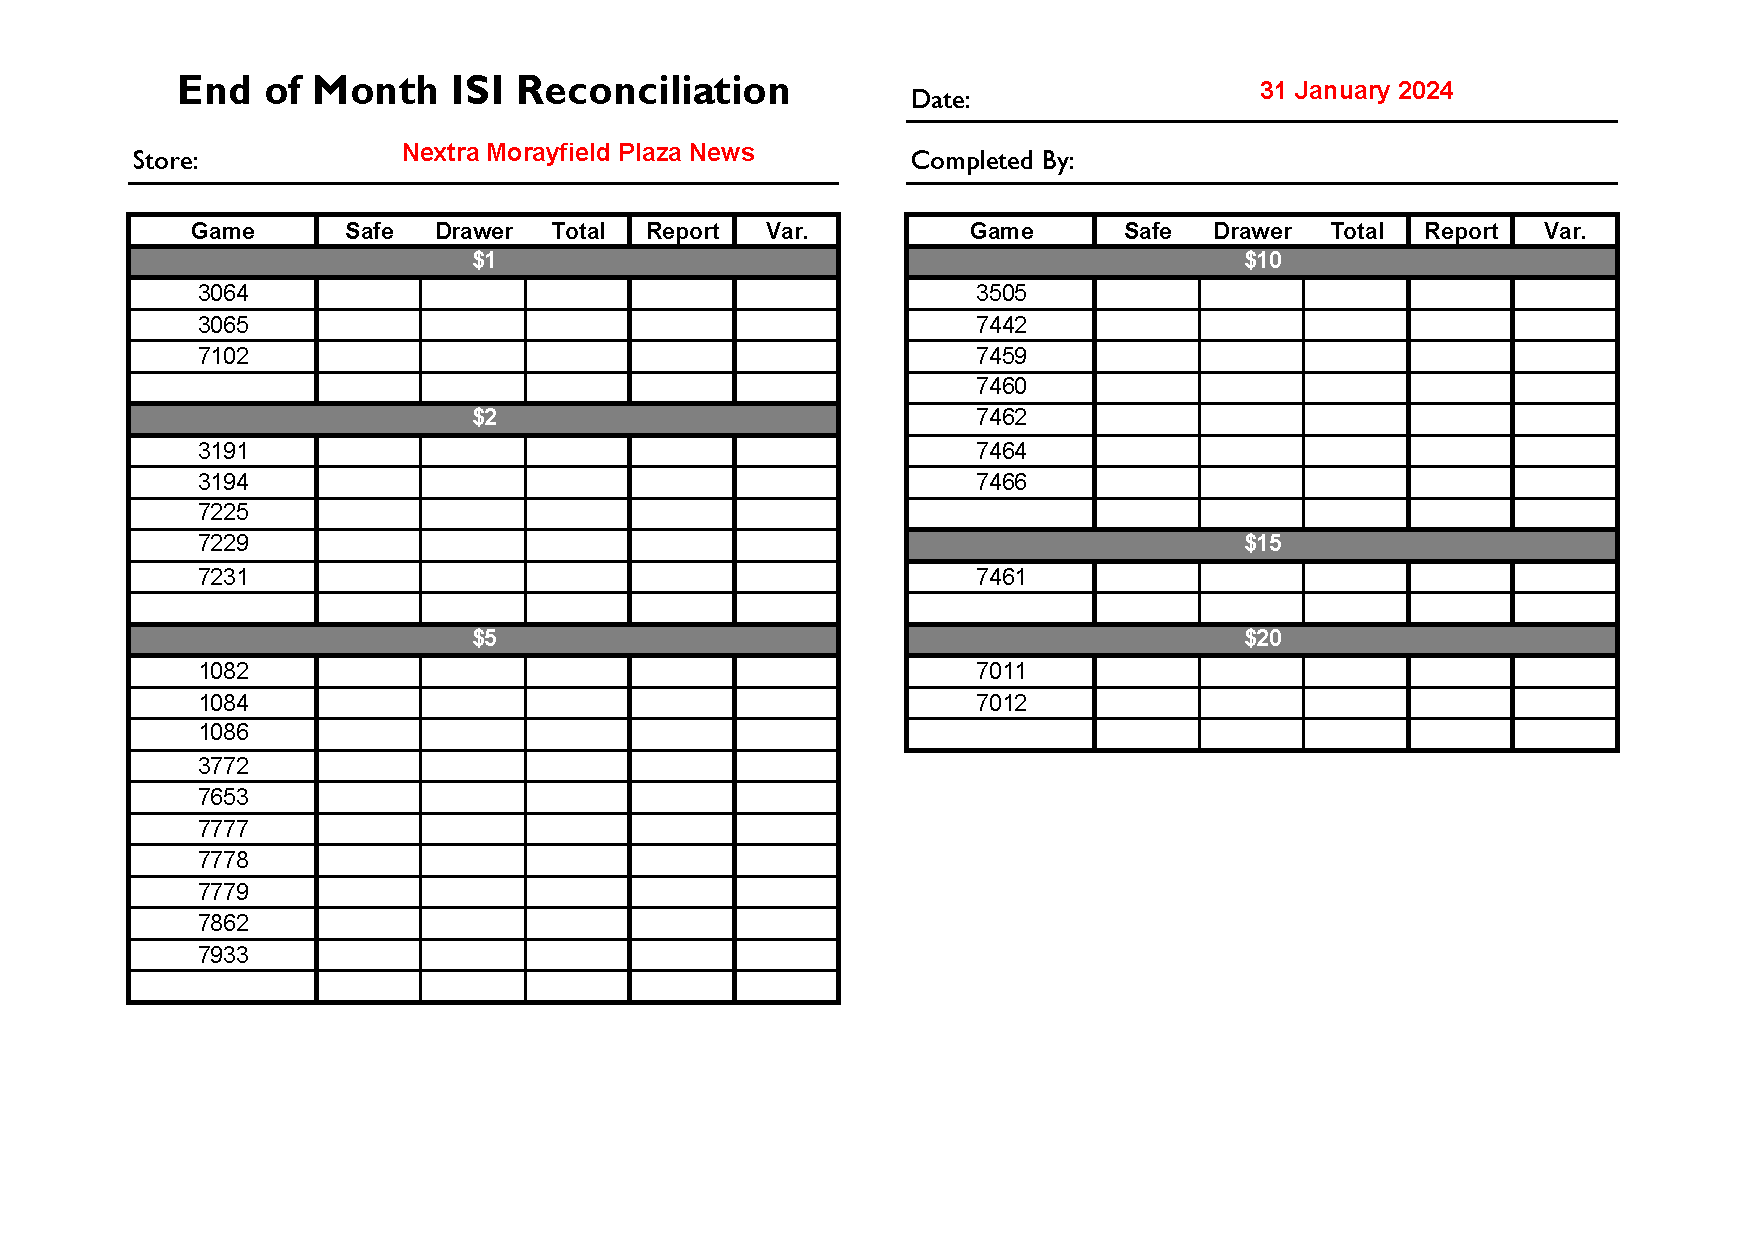
\includepdf[pages=-, landscape=true]{eomisirecon.pdf}

\end{document}
